\documentclass[presentation]{beamer}
%\documentclass[handout]{beamer}
\usetheme{Frankfurt}
\usecolortheme{seahorse}

\usepackage{amssymb}
\usepackage{amsmath}
\usepackage{graphicx}
\usepackage{subfig}
\usepackage{multicol}
\usepackage[font={footnotesize,it}]{caption}

\usepackage{tikz}
\usetikzlibrary{graphdrawing,graphs} 
\usegdlibrary{layered}
\usegdlibrary{force}
\usegdlibrary{trees}

\usepackage{hyperref}

\begin{document}

\title{Using Time Series Models for Defect Prediction in Software Release Planning}
\author{James Tunnell \\
Central Washington University \\
Computational Science Program}
\date{May 21, 2015}

\begin{frame}
\titlepage
\end{frame}

\begin{frame}
\small{
\frametitle{Outline}
\tableofcontents[hideallsubsections] 
}
\end{frame}

\section{Introduction}

\begin{frame}
\begin{center}
\Large{Introduction}
\end{center}
\end{frame}

\subsection{Release Planning}

\begin{frame}[t]
\frametitle{Release Planning Objectives}
\begin{itemize}
\item{Two primary objectives of software release planning are:
  \begin{itemize}
    \item{Improving functionality}
    \item{Maintaining quality}
  \end{itemize}}
  \item{Both of these objectives are constrained by limits on development time and cost.}
\end{itemize}
\end{frame}

\subsection{Quality Control}

\begin{frame}[t]
\frametitle{Quality Control}
\begin{itemize}
  \item{Software defects (bugs) are inevitable}
  \item{Sufficient time should be available to ensure good quality (by testing and bug-fixing)}
  \item{Otherwise, there is a risk of
    \begin{itemize}
    \item{Low quality (failure to meet objective)}
    \item{Schedule slip (failure to respect constraint)}
    \end{itemize}
  }
  \item{This quality control (QC) time can be allowed for by limiting the scope of work in the planned release}
\end{itemize}
\end{frame}

\begin{frame}[t]
\frametitle{Quality Control (cont'd)}
\begin{itemize}
  \item{To support release planning, QC time can be estimated}
  \item{Assumption: QC time depends (at least partly) on the number of software defects introduced}
  \item{Then, a basis for estimating QC time would be the predicted number of defects}
\end{itemize}
\end{frame}

\subsection{Defect Prediction}

\begin{frame}[t]
\frametitle{Defect Prediction}
\begin{itemize}
  \item{Approaches to defect prediction tend to focus on either
    \begin{itemize}
    \item{Code analysis
      \begin{itemize}
      \item{Lines of code}
      \item{Number of decisions}
      \item{Code churn}
      \end{itemize}
    }
    \item{Historical information
      \begin{itemize}
      \item{Regression analysis}
      \item{Time series modeling}
	  \end{itemize}
	}
    \end{itemize}
  }
  \item{A multivariate time series model with exogenous inputs was chosen}
\end{itemize}
\end{frame}

%\subsection{Related Work: Using Code Analysis}
%
%\begin{frame}[t]
%\frametitle{Defect Prediction using Code Analysis}
%\begin{itemize}
%\item{Approaches using code analysis:
%  \begin{itemize}
%  \item{Akiyama used lines of code (LOC), number of decisions, and the number of subroutine calls \cite{1971_akiyama}}
%  \item{Gafney also used LOC \cite{1984_gaffney_estimating}}
%  \item{Henry and Kafura use information taken from design documents \cite{1984_henry_evaluation}}
%  \item{Nagappan and Ball use relative code churn (lines modified) \cite{2005_nagappan_codechurn}}
%  \end{itemize}
%}
%\item{These approaches all depend on specific design or implementation information}
%\item{This information is not available at the release planning stage}
%\end{itemize}
%\end{frame}
%
%\subsection{Related Work: Using Historical Information}
%
%\begin{frame}[t]
%\frametitle{Defect Prediction using Historical Information}
%\begin{itemize}
%\item{Approaches using historical information:
%  \begin{itemize}
%  \item{Li et al. extrapolate parameters of a regression model \cite{2004_li_emperical_eval}}
%  \item{Singh et al. use an ARIMA time series model \cite{2010_singh_predicting}}
%  \end{itemize}
%}
%\item{Both approaches are non-specific to design or implementation}
%\item{However, neither approach is explanatory}
%\end{itemize}
%\end{frame}

\section{Motivation}

\begin{frame}
\begin{center}
\Large{Motivation}
\end{center}
\end{frame}

\subsection{Explanatory Model}

\begin{frame}[t]
\frametitle{Explanatory Model}
\begin{itemize}
\item{Assumption: the number of defects in the future depends on more than just the number of defects in the past}
\item{A defect prediction model that depends only on previous numbers of defects is not explanatory}
\item{Such a non-explanatory model would always predict the same number of defects}
\end{itemize}

\begin{figure}[htbp]
\begin{center}
\tikz[nodes={text height=1em, text depth=.2em, draw=black!20, thick, fill=white, font=\small}, rounded corners, semithick]
  \graph[layered layout, level distance = 1cm, sibling sep = 1em]{
    "Release Plan 1" -> "Non-explanatory Model";
    "Release Plan 2" -> "Non-explanatory Model";
    "...." -> "Non-explanatory Model";
    "Release Plan N" -> "Non-explanatory Model";
    "Non-explanatory Model" -> "Predicted Defects";
  };
\caption{A non-explanatory model.}
\end{center}
\end{figure}
\end{frame}


\begin{frame}[t]
\frametitle{Explanatory Model (cont'd)}
\begin{itemize}
\item{A model could also depend on the key factors of a release plan}
\item{This would be an explanatory model structure}
\item{Such a model can potentially predict a different number of defects for every release plan}
\end{itemize}

\begin{figure}[htbp]
\begin{center}
\tikz[nodes={text height=1em, text depth=.2em, draw=black!20, thick, fill=white, font=\small}, rounded corners, semithick]
  \graph[layered layout, level distance = 1cm, sibling sep = 1em]{
    "Release Plan 1" -> "Explanatory Model";
    "Release Plan 2" -> "Explanatory Model";
    "...." -> "Explanatory Model";
    "Release Plan N" -> "Explanatory Model";
    "Explanatory Model" -> "Predicted Defects 1";
    "Explanatory Model" -> "Predicted Defects 2";
    "Explanatory Model" -> "...";
    "Explanatory Model" -> "Predicted Defects N";
  };
\caption{An explanatory model.}
\end{center}
\end{figure}
\end{frame}

\section{Time Series}

\begin{frame}
\begin{center}
\Large{Time Series Modeling}
\end{center}
\end{frame}


\subsection{Time Series}

\begin{frame}[t]
\frametitle{Time Series }
\begin{itemize}
\item{A time series is a collection of observations that occur in order}
\item{The process underlying a time series is assumed to be stochastic (non-deterministic)}
\item{Each observation might depend on one or more previous observations}
\item{This dependence is termed \textit{autocorrelation}}
\end{itemize}
\end{frame}

\subsection{Autoregressive Models}

\begin{frame}[t]
\frametitle{Autoregressive Models}
\begin{itemize}
\item{A basic autoregressive (AR) model is a linear combination of previous values}
\item{A white noise term accounts for stochastic fluctuation}
\item{An $AR(p)$ model for predicting a value X at time t is
\begin{equation}
X_t=c+\sum_{i=1}^{p}{\phi_i X_{t-i}+\epsilon_t}
\end{equation}
where $\phi_1, \phi_2, ..., \phi_p$ are the $p$ parameters, $c$ is a constant, and $\epsilon_t$ is the white noise term}
\end{itemize}
\end{frame}

\begin{frame}[t]
\frametitle{Autoregressive Models (cont'd)}
\begin{itemize}
\item{Extending the AR model to be multivariate results in a Vector AR (VAR) model}
\item{This model can support time series for defect count, improvements, and new features}
\end{itemize}
\end{frame}

\subsection{More on Modeling}

\begin{frame}[t]
\frametitle{More on Modeling}

\large{Endogeneity vs Exogeneity}
\begin{itemize}
\item{Endogeneity vs Exogeneity
  \begin{itemize}
  \item{We only attempt to explain the number of defects, so all other model inputs are exogenous.}
  \item{This makes a VAR model would become a VARX model}
  \end{itemize}
}
\item{Stationarity
  \begin{itemize}
  \item{The models discussed so far require stationary time series data}
  \item{Statistical tests are applied to check for stationarity}
  \item{Non-stationary time series are differenced}
  \end{itemize}
}
\end{itemize}
\end{frame}

\section{Modeling Methodology}

\begin{frame}
\begin{center}
\Large{Modeling Methodology}
\end{center}
\end{frame}

\subsection{Overview}

\begin{frame}[t]
\frametitle{Time Series Modeling Methodology}
\begin{itemize}
\item{Time series modeling methodology typically involves
  \begin{enumerate}
  \item{Specification}
  \item{Estimation}
  \item{Diagnostic Checking}
  \item{Selection}
  \end{enumerate}}
\end{itemize}
\end{frame}

\subsection{Specification \& Estimation}

\begin{frame}[t]
\frametitle{Specification \& Estimation}
\begin{itemize}
\item{A $VARX(p)$ model is specified by choosing an order $p$}
\item{Model order is the number of autoregressive terms}
\item{This affects the number of parameters included in the model}
\item{The model order is limited to avoid having too many parameters relative to the number of observations}
\item{Maximum model order is $p_max$}
\item{Models parameters are estimated for orders $1, 2,..., p_{max}$}
\end{itemize}
\end{frame}


\subsection{Diagnostic Checking}

\begin{frame}[t]
\frametitle{Diagnostic Checking}
\begin{itemize}
\item{Diagnostics can tell if a model should be rejected}
\item{First diagnostic is for stability
  \begin{itemize}
  \item{AR model can have infinite impulse response}
  \item{To be stable, the roots of the characteristic equation must lie outside the unit circle}
  \item{Equivalently, the inverse of the roots must lie inside the unit circle}
  \end{itemize}
}
\item{Next diagnostic is residual autocorrelation
  \begin{itemize}
    \item{Model residuals should be indistinguishable from white noise}
    \item{White noise is uncorrelated (no autocorrelation)}
    \item{Ljung-Box test forms a statistic from the autocorrelation of the residuals}
  \end{itemize}
}
\end{itemize}
\end{frame}

\subsection{Model Selection}

\begin{frame}[t]
\frametitle{Model Selection}
\begin{itemize}
\item{Model selection criteria are used to compare models according to their fit}
\item{Penalties for residual error and the number of parameters}
\item{Some common selection criteria
  \begin{itemize}
  \item{Akaike Information Criterion (AIC)}
  \item{AIC with correction (AICc)}
  \item{Bayesian Information Criterion (BIC)}
  \end{itemize}
}
\item{Parameter penalty is more severe for BIC and AICC than for AIC}
\item{AIC will be used, since the number of parameters is already limited in the specification step}
\end{itemize}
\end{frame}

\section{Data Methodology}

\begin{frame}
\begin{center}
\Large{Data Methodology}
\end{center}
\end{frame}

\note{In this section, the data source and data collection method are detailed. Then, the method of preparing data for the modeling phase is presented.}

\subsection{Data Source}

\begin{frame}[t]
\frametitle{Data source}
\begin{itemize}
\item{Data for time series modeling will be derived from project historical data}
\item{This historical data can be found in the project issue tracking system (ITS)}
\item{The issues in an ITS can be bugs, features, improvements, etc.}
\item{The \textit{MongoDB} software project was selected to try out the modeling methodology
\begin{itemize}
\item{The project has been actively developed since 2009}
\item{Data from versions 0.9.3 through 3.0.0-rc6 are used}
\item{This dataset contained $7042$ issues}
\end{itemize}
\item{Only data on issues leading to software changes were kept.}
}
\end{itemize}
\end{frame}

\subsection{Data Preparation}

\begin{frame}[t]
\frametitle{Data Sampling}
\begin{itemize}
\item{Time series data was drawn for the issue data by
  \begin{itemize}
  \item{Sampling}
  \item{Testing for stationarity}
  \item{Windowing samples to limit exposure to underlying process changes}
  \end{itemize}
}
\item{A 78-week time window (approximately 18 months) was chosen}
\item{This window was applied over all the data by a sliding window}
\item{Modeling methodology is applied to each window}
\end{itemize}
\begin{figure}[htbp]
\begin{center}
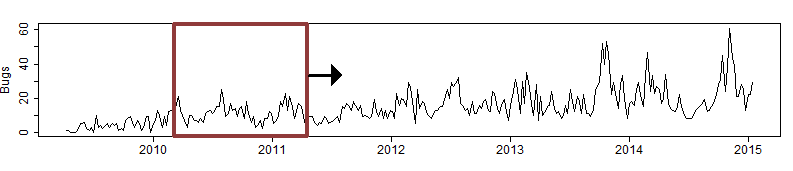
\includegraphics[width=\textheight]{assets/time_series_sliding_window.png}
\caption{Sliding time window moves over the entire time series.}
\end{center}
\end{figure}
\end{frame}

\section{Results}

\begin{frame}
\begin{center}
\Large{Results}
\end{center}
\end{frame}

\subsection{Data Methodology}

\begin{frame}[t]
\frametitle{\textit{MongoDB} Time Series Data}
Time series data was obtained by sampling the \textit{MongoDB} dataset with a 7-day sample period
\begin{figure}[htbp]
\begin{center}
\includegraphics[height=.6\textheight]{assets/time_series.eps}
\caption{\textit{MongoDB} time series data}
\end{center}
\end{figure}
\end{frame}

\begin{frame}[t]
\frametitle{Stationarity \& Differencing}
\footnotesize{
\begin{itemize}
\item{At first, ADF and KPSS test results disagreed}
\item{After differencing, test results agreed}
\end{itemize}
}
\vspace{-.5cm}
\begin{figure}[htbp]
\begin{center}
\includegraphics[height=.6\textheight]{assets/time_series_diff.eps}
\caption{\textit{MongoDB} time series data after differencing}
\end{center}
\end{figure}
\end{frame}

\subsection{Modeling Methodology}

\begin{frame}[t]
\frametitle{One-step Predictions}
\small{One-step predictions are a visual indication of model fit. Here are the one-step predictions for three of the models.}

\begin{figure}[htbp]
\centering
\vspace{-.25in}
\subfloat{
\includegraphics[width=.65\textwidth]{assets/one-step_predictions_2-79.eps}
}\\
\vspace{-.6in}
\subfloat{
\includegraphics[width=.65\textwidth]{assets/one-step_predictions_80-157.eps}
}\\
\vspace{-.6in}
\subfloat{
\includegraphics[width=.65\textwidth]{assets/one-step_predictions_158-235.eps}
}%
\caption{Actual values (solid) vs. one-step predictions (dotted)	}
\end{figure}
\end{frame}


\subsection{Forecasting}

\begin{frame}[t]{Sliding Window Forecasts}
\begin{itemize}
\item{How useful is the VARX model in general, considering these conflicting results?}
\item{To find out, a sliding 78-week window was used}
\item{The sliding window started at the first sample period, and was shifted by one sample period after modeling}
\item{Only the actual number of improvements and features were used in this forecasting}
\end{itemize}
\end{frame}

\begin{frame}[t]{Sliding Window Forecasts (cont'd)}
\footnotesize{
\begin{itemize}
\item{Errors between the mean forecasted and actual number of bugs is shown as a histogram}
\item{The histogram appears to be normally distributed (good)}
\item{The variability is quite large (bad)}
\item{The actual number of bugs was inside the 90\% confidence interval for 23.87\% of the sliding window ranges}
\end{itemize}
\vspace{-.5cm}
\begin{figure}[htbp]
\begin{center}
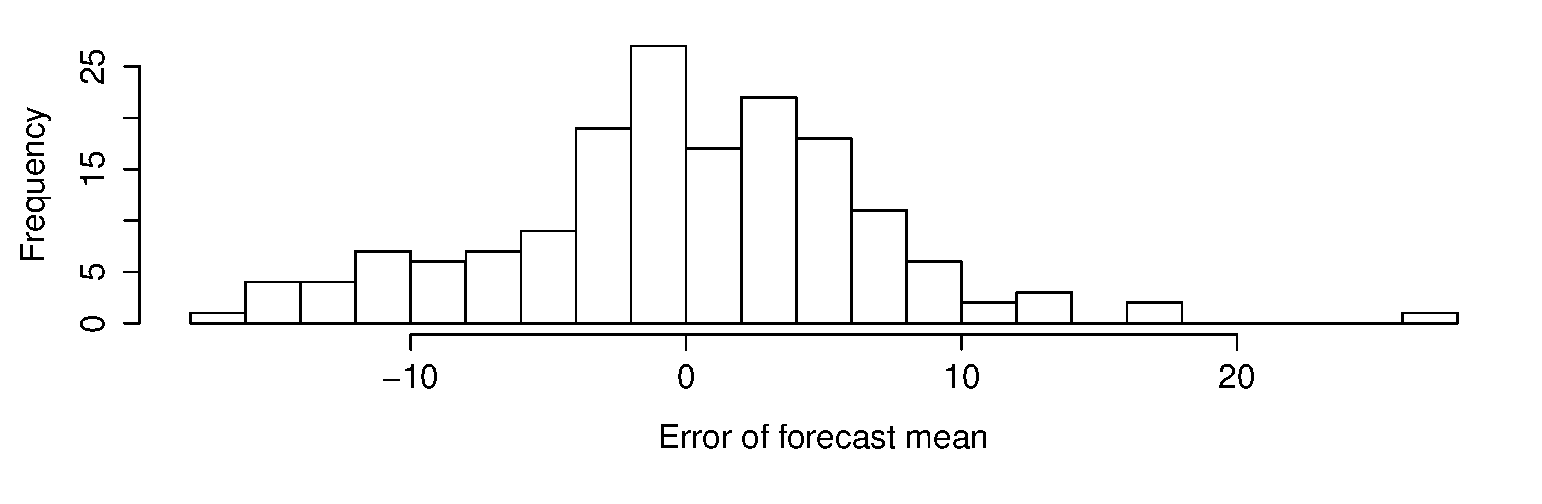
\includegraphics[width=.9\textwidth]{assets/forecast_errors.eps}
\caption{Histogram of errors in forecast mean obtained using a 78-week sliding window.}
\end{center}
\end{figure}
}
\end{frame}


\section{Conclusions}

\begin{frame}
\begin{center}
\Large{Conclusion \& Future Work}
\end{center}
\end{frame}

\subsection{Conclusions}

\begin{frame}[t]{Conclusions}
\footnotesize{
\begin{itemize}
\item{The VARX modeling methodology was successfully applied to the time series data collected from the \textit{MongoDB} project}
\item{Models were created for each of three time windows}
\item{A model was selected for each window}
\item{Forecast results using the models were inconclusive}
\item{A better picture of the prediction performance was obtained using a sliding window}
\item{This resulted in a normally distributed error in the mean forecasted values}
\item{A low proportion (23.87\%) of the sliding window ranges included the actual number of bugs in the 90\% confidence interval}
\item{These results may indicate that a VARX model will not be useful to make predictions for the the MongoDB dataset}
\end{itemize}
}
\end{frame}

\subsection{Future Work}

\begin{frame}{Future Work}
Having applied the VARX time series model to one project dataset, a next step is to apply the methodology to other software project data sets, such as \textit{Eclipse} or \textit{Mozilla}, to more conclusively determine the model's usefulness.
\end{frame}

\end{document}
